\documentclass[14pt, a4paper]{extarticle}
    \usepackage[mathletters]{ucs} % Extended unicode (utf-8) support
    \usepackage[X2,T2A]{fontenc}
    \usepackage[utf8]{inputenc} % Allow utf-8 characters in the tex document
	\usepackage[left=25mm, right=25mm, top=20mm, bottom=20mm]{geometry}
	\usepackage[hyphens]{url}
   	\usepackage[hidelinks, linktoc=all,russian]{hyperref}
	\usepackage{indentfirst}
	\usepackage{hyphenat}
    \usepackage{subcaption}
   	\usepackage[biblabel]{cite}
    \usepackage[font=small,labelfont=bf]{caption}
    \usepackage{abstract}
    \usepackage{mathtools}
    \usepackage[resetlabels,labeled]{multibib}
    \usepackage[english,main=russian]{babel}
    \usepackage{babelbib}

    \usepackage{mathrsfs}  
    \usepackage{fontawesome}
    \usepackage{cleveref}
    \usepackage{fancyhdr}
    \usepackage{qrcode}
    \usepackage{enumitem}
    \setlength{\parskip}{0.1cm}   
	\setlength{\parindent}{0.7cm}
	\usepackage{setspace}
	\onehalfspacing
    \usepackage{graphicx} % Used to insert images
    \usepackage{adjustbox} % Used to constrain images to a maximum size 
   	\usepackage{color} % Allow colors to be defined
    \usepackage{amsmath} % Equations
    \usepackage{amssymb} % Equations
	\usepackage{kbordermatrix}

    \usepackage{grffile} 
    \usepackage{tabularx}
	\usepackage{bbm}
	\usepackage{booktabs}
	\usepackage{multirow}
	\usepackage{makecell} 
	\usepackage{titlesec}
	
	\titleformat{\chapter}
	{\normalfont\fontsize{20}{24}\bfseries}{\thechapter}{1em}{}
	
	
	\titleformat{\section}
	{\normalfont\fontsize{16}{20}\bfseries}{\thesection}{1em}{}
	\titleformat{\subsection}
	{\normalfont\fontsize{14}{16}\bfseries}{\thesubsection}{1em}{}


\newcommand{\diff}{\,\mathrm{d}} 	
 	
 \addto\extrasrussian{%
 	\renewcommand{\figureautorefname}{Рис.}%
 	 \renewcommand{\tableautorefname}{Таб.}%
 }

\renewcommand*\thesection{\arabic{section}}
\DeclarePairedDelimiter\bra{\langle}{\rvert}
\DeclarePairedDelimiter\ket{\lvert}{\rangle}
\DeclarePairedDelimiterX\braket[2]{\langle}{\rangle}{#1 \delimsize\vert #2}
\newcommand{\rbrkt}[1]{\left( #1 \right)}
\newcommand{\sbrkt}[1]{\left[ #1 \right]}
\newcommand{\rot}{\text{\textbf{rot}}\,}
\newcommand{\Tr}{\text{Tr}}


\setcounter{tocdepth}{3}


\renewcommand*\thesection{\arabic{chapter}.\arabic{section}}
\lhead[\rm\thepage]{\fancyplain{}{\nouppercase{\sl{\rightmark}}}}
\rhead[\fancyplain{}{\nouppercase{\sl{\leftmark}}}]{\rm\thepage}
\chead{}\lfoot{}\rfoot{}\cfoot{}
\pagestyle{plain}

\DeclareUnicodeCharacter{0462}{\CYRYAT}\DeclareTextSymbolDefault{\CYRYAT}{X2}\DeclareUnicodeCharacter{0463}{\cyryat}\DeclareTextSymbolDefault{\cyryat}{X2}

\graphicspath{{Pictures/}}

\newcites{A}{Основные публикации по теме диссертации}


\begin{document}

\selectlanguage{russian}
\begin{titlepage}

\vspace*{0.2cm}
\begin{flushright}
На правах рукописи\\
УДК 539.12
\end{flushright}

\vfill

\begin{center}
Федоров Глеб Петрович

\vspace*{0.5cm}

{\large Моделирование квантового взаимодействия излучения и вещества с использованием массивов сверхпроводниковых искусственных атомов}


\begin{center}
01.04.07 --- физика конденсированного состояния\\
\end{center}


\vspace*{2cm}


\begin{center}
АВТОРЕРЕФЕРАТ\\
диссертации на соискание ученой степени\\
кандидата физико-математических наук
\end{center}



\vfill

Долгопрудный --- 2021
\end {center} 
\end{titlepage}

\setcounter{page}{2}
\noindent Работа прошла апробацию в лаборатории искусственных квантовых систем федерального государственного автономного образовательного учреждения высшего образования <<Московский физико-технический институт (национальный исследовательский университет)>>

\vspace{1.5cm}
\noindent\begin{tabular*}{1.02\textwidth}{l@{\extracolsep{\fill}}r}
\textbf{Научный руководитель:}&\begin{tabular}[t]{r}
	Рязанов Валерий Владимирович,\\
	доктор физико-математических наук,\\
	профессор\end{tabular}
\end{tabular*}

\vspace{1.5cm}
\noindentВедущая организация: федеральное государственное бюджетное учреждение науки Институт проблем химической физики Российской академии наук (ИПХФ РАН)

\vspace{1.5cm}
\noindentЗащита состоится << >> сентября 2021 года в 16:00 на заседании диссертационного совета ЛФИ.01.04.07.007 по адресу: 141801, Московская область, г. Долгопрудный, Институтский пер., 9.

\vspace{1.5cm}
\noindentС диссертацией можно ознакомиться в библиотеке и на сайте Московского физико-технического института (национального исследовательского университета) \url{https://mipt.ru/education/post-graduate/soiskateli-fiziko- matematicheskie-nauki.php}

\vspace{1.5cm}
\noindentРабота представлена << >> мая 2021 г. в Аттестационную комиссию федерального государственного автономного образовательного учреждения высшего образования <<Московский физико-технический институт (национальный исследовательский университет)>> для рассмотрения советом по защите диссертаций на соискание ученой степени кандидата наук, доктора наук в соответствии с п. 3.1. ст. 4 Федерального закона <<О науке и государственной научно-технической политике>>.

\section*{Общая характеристика работы}

\textbf{Актуальность работы.} История развития сверхпроводниковых искусственных атомов, или кубитов, как инструмента для наблюдения макроскопических квантовых эффектов берет своё начало в 1997 году, когда в группе проф. Накамуры в Японии была впервые показана когерентность суперпозиции зарядовых состояний одноэлектронного транзистора \cite{nakamura1997spectroscopy}. Этот эксперимент стал толчком к развитию новой области физики, интерес к которой обеспечивался как открывшимися возможностями изучать фундаментальные физические явления, так и потенциальной применимостью для квантовых вычислений.

Несмотря на относительно недавнее появление, сверхпроводниковые или, как их также называют, джозефсоновские кубиты прошли уже много стадий в своем развитии. Системы, исследовавшиеся в первых экспериментах, имели очень низкие времена когерентности: например, в работе \cite{nakamura1999coherent} время затухания Раби-осцилляций в зарядовом кубите составило около 1 нс. Сейчас стандартные времена когерентности составляют для ведущих групп порядка 100 микросекунд \cite{kjaergaard2020superconducting}. Наиболее далеко в области квантовых вычислений продвинулись американские учёные, работающие теперь в компаниях Google и IBM. В частности, в 2019 году Google продемонстрировала квантовое превосходство своего процессора из 53 кубитов над мощнейшим существующим классическим компьютером \cite{arute2019quantum}. Однако даже этот результат пока ещё далёк от реальных практических применений, так как количество ошибок, происходящих в устройстве, по-прежнему еще очень велико, а решаемая задача была создана искусственно для минимизации чувствительности результата к декогеренции. Как было показано П. Шором еще в конце прошлого столетия \cite{shor1995scheme}, практические квантовые вычисления потребуют реализации алгоритмов коррекции ошибок, что неминуемо потребует существенного увеличения числа физических кубитов для обеспечения работы небольшого числа логических. Увеличение же числа кубитов более, чем на порядок, непременно натолкнётся на трудности масштабирования контролирующей электроники и криогенной аппаратуры \cite{krinner2019engineering}, алгоритмов калибровки системы \cite{arute2019quantum, kelly2018physical}, а также проектирования самих сверхпроводящих интегральных схем \cite{hutchings2017tunable}. Отсюда следует, что сегодня нельзя назвать даже примерных сроков реализации практически полезных квантовых алгоритмов \cite{arute2019quantum}.

Однако острый интерес к потенциальным применениям в области квантовых вычислений мотивировал исследования на основе сверхпроводящих кубитов и по другим направлениям \cite{kjaergaard2020superconducting}. В частности, чрезвычайно большое количество экспериментов было проведено в области квантовой электродинамики цепей \cite{blais2020quantum}, вдохновленной нобелевскими исследованиями С. Ароша \cite{haroche2013nobel} по стандартной квантовой электродинамике полостей. Впервые сверхпроводниковый искусственный атом был сильно связан с квантованным полем в резонаторе в 2004 году в Йельском университете \cite{wallraff2004strong}, что стало первым в истории экспериментальным подтверждением возможности связать одиночную квантовую систему с полем так, чтобы сила связи превысила диссипацию. С развитием технологии производства алюминиевых сверхпроводниковых чипов, открытием новых схем расположения их элементов, а также удешевлением электроники все больше групп в мире стали включаться в работу и вести собственные исследования. В Йельском университете работают проф. Деворе (Michel Devoret) и проф. Шелькопф (Robert Schoelkopf), занимающиеся, в основном, экспериментами с неклассическими состояниями света в микроволновых резонаторах, которые они готовят, используя связанные с ними искусственные атомы (см. \cite{vlastakis2013deterministically, mirrahimi2014dynamically}). В этой группе также берут начало известные работы компании IBM (см. \cite{jurcevic2020demonstration}), а также стартап Rigetti, по фамилии одного из защитившихся в Йельском университете аспирантов \cite{reagor2018demonstration}. В группе проф. Мартиниса (John Martinis) в университете Калифорнии, Санта Барбара, помимо обширной работы по развитию квантовых алгоритмов \cite{arute2019quantum}, проводились исследования многочастичной локализации \cite{chen2014emulating, roushan2017spectroscopic}, квантового хаоса. В группе проф. Сиддики (Irfan Siddiqi), университет Калифорнии, Бёркли, проводятся эксперименты по наблюдению и изучению отдельных квантовых траекторий и квантовых скачков, которые испытывает кубит под воздействием сильных или слабых измерений (см. \cite{hacohen2016quantum} и ссылки там же). Проф. Астафьев, работавший в Японии и затем в Англии, провёл первые эксперименты по взаимодействию свободного излучения в волноводах с джозефсоновскими кубитами \cite{astafiev2010resonance}. Проф. Устинов в университете Карлсруэ руководил экспериментами по исследованию двухуровневых туннельных дефектов \cite{grabovskij2012strain}, мультиплексированному по частоте дисперсионному считыванию \cite{jerger2012frequency}, реализации квантовых метаматериалов \cite{macha2014implementation}. В Дельфтском университете под руководством проф. Ди Карло (Leonardo Di Carlo) проводились одни из первых экспериментов по реализации квантовых алгоритмов на двухкубитных схемах, а затем изучалась возможность цифрового моделирования произвольных гамильтонианов \cite{langford2017experimentally}. Проф. Ильичев в университете фотоники Йены проводил первые эксперименты для компании DWave со связанными потоковыми кубитами \cite{grajcar2006four}. Проф. Рязанов занимался разработкой и исследованиями кубитов с джозефсоновскими $\pi$-контактами \cite{feofanov2010implementation}. Наконец, в группе проф. Вальрафа (Andreas Wallraff) проводятся эксперименты с одиночными микроволновыми фотонами, например, по созданию источника последовательности перепутанных друг с другом фотонов \cite{besse2020realizing} или использованию одиночных летящих фотонов для перепутывания удаленных кубитов \cite{kurpiers2018deterministic}.

Как можно видеть, с течением времени обнаружился обширный перечень областей применения сверхпроводниковых квантовых систем, без которых все приведенные выше эксперименты были бы невозможны. Исследования, описанные в данной диссертации, посвящены экспериментальной реализации взаимодействия излучения и вещества в квантовом режиме при помощи сверхпроводниковых искусственных атомов. Данная тема лежит за пределами области цифровых квантовых вычислений и скорее оказывается ближе к аналоговому моделированию одних квантовых систем другими в духе изначального предложения Р. Фейнмана \cite{feynman1982simulating}. Известно, что системы связанных кубитов позволяют экспериментально реализовывать симуляторы спиновых массивов в квантовом режиме, что пытается использовать в своих машинах компания DWave (см, например, \cite{harris2018phase}): однозначное отображение спинового гамильтониана на экспериментальный образец дает надежду на то, что измерение параметров физической системы позволит найти положение минимума энергии в пространстве конфигураций модельного гамильтониана. Подобным образом в ходе мировых исследований было выявлено, что системы связанных многоуровневых кубитов\hyp трансмонов подходят для аналогового моделирования гамильтониана Бозе-Хаббарда \cite{Orell2019, Ma2019, Hacohen-Gourgy2015, Deng2016, Ye2019, Yan2019}. Такое соответствие открывает целое направление экспериментальных исследований, так как по сути соединяет сверхпроводниковые когерентные системы с различными областями теоретической и экспериментальной физики, использующими ту же математическую модель.

\paragraph{Цель работы.} Целью диссертационной работы являются экспериментальные и теоретические исследования возможностей аналогового моделирования взаимодействия излучения и вещества при помощи квантовых сверхпроводниковых устройств, а также поиск и описание новых эффектов возникающих при таком взаимодействии.

Для достижения поставленной цели в ходе исследований были сформулированы следующие \textbf{задачи}:

\begin{enumerate}
		\item Создание экспериментальной базы для исследования сверхпроводниковых квантовых систем, разработка программной системы автоматизации измерений.
	\item Исследование времен когерентности образцов, содержащих одиночные кубиты, связанные с микроволновыми резонаторами, с целью контроля и улучшения их характеристик при изготовлении
	\item Численное моделирование системы двух связанных кубитов\hyp трансмонов (сверхпроводниковой искусственной молекулы), расчет уровней энергии в трехуровневом приближении, расчет электромагнитных параметров системы, создание технологических чертежей.
	\item Экспериментальное исследование образца, изготовленного по созданным чертежам, при криогенных температурах. Сопоставление результатов с численной моделью, подробное изучение влияния эффектов гибридизации на форму спектральных линий многофотонных переходов при использовании сигналов накачки большой мощности, теоретическое описание наблюдаемых эффектов.
	\item Численное моделирование цепочки, состоящей из пяти кубитов\hyp трансмонов, путем решения основного кинетического уравнения для эволюции матрицы плотности подсистемы. Исследование её поведения в двухуровневом приближении (спиновой динамики), в классическом линейном пределе, расчет матрицы емкостей с учетом подключения СВЧ-волноводов, создание технологических чертежей.
	\item Проведение спектроскопии пропускания цепочки векторным анализатором цепей при криогенных температурах, получение зависимости мнимой и действительной части комплексного коэффициента рассеяния от частоты и от мощности падающего сигнала. Сравнение экспериментальных данных с результатами теоретического расчета по теории отклика (input\hyp output), описание и объяснение отличий спектров от предсказаний классической электродинамики. Изучение статистики энергетических уровней системы и исследование влияния управляемого беспорядка в энергиях трансмонов на её транспортные свойства.
\end{enumerate}



\paragraph{Основные положения, выносимые на защиту.}

\begin{enumerate}
	\item Разработанные методы компьютерного зрения позволяют осуществлять детектирование результатов однотоновой и двухтоновой спектроскопии и с хорошей точностью извлекать параметры кубитов-трансмонов для осуществления полностью автоматических измерений.
	\item Разработана и экспериментально исследована система из двух связанных кубитов\hyp трансмонов, построена квантовомеханическая модель, предсказывающая и объясняющая как наблюдаемые спектральные линии, так и необычные эффекты из-за гибридизации системы с падающим на нее излучением.
	\item Разработана и экспериментально исследована цепочка из пяти кубитов\hyp трансмонов, моделирующая фотонный транспорт через гамильтониан Бозе\hyp Хаббарда, связанный с резервуарами на его краях; построена теоретическая модель, позволяющая численно рассчитать неравновесную динамику с учетом диссипации и внешнего вынуждения и предсказывающая спектральные свойства системы; показан переход от классического линейного режима к нелинейному, квантовому режиму работы системы с увеличением мощности падающего излучения. Экспериментально исследовано подавление транспорта фотонов путем введения управляемого беспорядка в энергии трансмонов.
\end{enumerate}
	
\paragraph{Научная новизна исследований.} Впервые были применены методы машинного зрения к задаче автоматизации измерений сверхпроводниковых квантовых устройств, что позволило проводить полный цикл экспериментов с однокубитными (для кубитов\hyp трансмонов) образцами без участия оператора.

Впервые проведено экспериментальное исследование и  подробный анализ многофотонных переходов в системе двух связанных кубитов\hyp трансмонов, возникающих при большой интенсивности накачки, впервые были обнаружены необычные проявления гибридизации излучения и вещества в составной системе, подобные эффекту Отлера\hyp Таунса, которые значительно изменяют структуру энергетических уровней системы. Построены самосогласованные теоретические модели для описания эффектов.

Впервые был экспериментально продемонстрирован прямой транспорт фотонов в через цепочку из пяти связанных кубитов\hyp трансмонов, впервые показан переход от классического режима транспорта к квантовому режиму фотонной блокады; продемонстрированы многофотонные переходы на многочастичные возбужденные состояния, точно предсказанные теоретическим расчетом. Экспериментально показано, что управляемый беспорядок, внесенный в систему, подавляет пропускание и свидетельствует о наступлении многочастичной локализации в цепочке.


\paragraph{Научная и практическая значимость работы.} Исследование сложных квантовых систем представляет значимость для современной науки и техники. Находясь на переднем крае физики, исследования по созданию и контролю многочастичных квантовых систем могут в конечном итоге привести к созданию практически полезных макроскопических квантовых устройств, которые найдут применение в решении задач материаловедения, машинного обучения, оптимизации и криптографии. Принципиальная сложность численного расчета квантовой системы, выражающаяся в экспоненциальном росте гильбертова пространства состояний с увеличением числа её подсистем, является с одной стороны проблемой, а с другой стороны -- возможностью, которую современной науке требуется использовать в своих целях. Эксперименты, проведенные диссертантом в рамках данной диссертации подтверждают, что контроль небольших по размеру систем возможен, и применение их для моделирования известных гамильтонианов действительно имеет перспективы. Исследования и методики, описанные в диссертации, будут служить основой для дальнейшего увеличения числа кубитов на образце, совершенствования архитектуры чипов, масштабирования измерительных установок и поиска новых применений и задач, для которых возможно будет использовать сверхпроводниковые квантовые технологии.


\paragraph{Апробация работы.} Основные результаты, полученные в диссертационной работе, докладывались на следующих профильных российских и международных конференциях:
\begin{itemize}
	\item 4-я международная конференция по квантовым технологиям, Москва, Россия, 12-16 июля 2017 (стендовый доклад)
	\item 1-я конференция по квантовым технологиям, Эстосадок, Россия, 1-7 марта 2018 (стендовый доклад)
	\item 2-я конференция по квантовым технологиям, Эстосадок, Россия, 1-7 марта 2019 года (стендовый доклад)
	\item 20-й зимний семинар физического факультета Института Технологий Карслруэ, Миттльберг, Австрия,  17-25 марта 2019 (устный доклад)
	\item 3-я международная конференция по квантовым технологиям, Эстосадок, Россия, 1-7 марта 2020 (стендовый доклад)
	\item 2-я ежегодная конференция по квантовым вычислениям, Эстосадок, Россия, 19-26 февраля 2021 (устный доклад)
\end{itemize}

\paragraph{Публикации.} По материалам диссертации опубликовано \textbf{5} печатных работ. Из них 5 статей в журналах, входящих в базы цитирования Scopus и Web of Science. 

\paragraph{Личный вклад автора.} Основные результаты, изложенные в данной диссертации, получены лично диссертантом или при его непосредственном участии. Во всех случаях
заимствования материалов других авторов в диссертации приведены ссылки
на литературные источники.

\paragraph{Достоверность} представленных в диссертационной работе результатов подтверждается соответствием между моделированием, аналитическими результатами и непосредственно полученными экспериментальными данными. Экспериментальные методы, использованные диссертантом, широко применяются в мировом научном сообществе; в работе приводятся соответствующие ссылки на печатные работы. Точность экспериментальных данных обеспечивается заводской калибровкой использованного коммерчески доступного оборудования.

\paragraph{Структура и объем работы.} Диссертация состоит из введения, трех глав и заключения. Она изложена на 185 страницах машинописного текста, включает 36 рисунков и 4 таблицы. Список литературы насчитывает 257 наименований.

\section*{Краткое содержание диссертации}

\paragraph{Во введении} обоснована актуальность темы диссертации, указаны ее цели, научная новизна, практическая значимость, структура и объем.

\paragraph{Первая глава} диссертации представляет собой литературный обзор тем, составляющих фундамент проведенных диссертантом исследований. Описаны на продвинутом уровне основы квантовой механики применительно к квантованию произвольных электрических цепей на примере планковского оциллятора, рассмотрены в этом контексте вопросы канонических преобразований и теории представлений. Также дан исторический обзор развития математического аппарата и физического понимания принципов квантовой механики по оригинальным работам. В качестве демонстрации применения теории Деворе к составлению лагранжианов цепей разобраны некоторые нетривиальные конфигурации элементов, приводящие к не поддающимся численному решению уравнениям Шредингера. 

Далее в историческом контексте рассматриваются эффекты сверхпроводимости и эффект Джозефсона. Приводится подробный обзор литературы в хронологическом порядке, от теории Лондонов до теории БКШ, показываются проблемы и пути их решения, важнейшие экспериментальные результаты, альтернативные теории, не получившие дальнейшего развития. Показан путь открытия эффекта Джозефсона, показаны трудности при установлении туннельного слагаемого гамильтониана для электронов, приведен краткий анализ математического аппарата и строгих результатов для критического тока стационарного эффекта и вывода уравнения нестационарного. 

\begin{figure}[t]
	\centering
	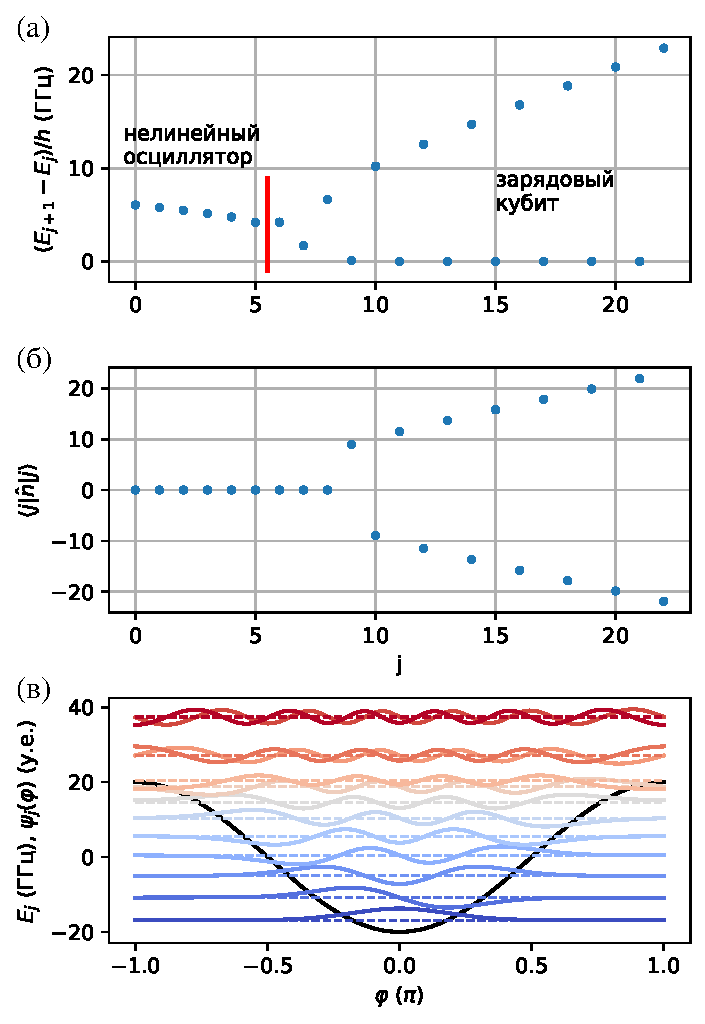
\includegraphics[width=0.6\linewidth]{Pictures/transmon_levels}
	\caption{(а) Разности энергий последовательных собственных состояний трансмона для $E_C/h = 250$ МГц, $E_J/h = 20$ ГГц. По линейному росту в правой части можно идентифицировать квадратичный закон дисперсии. (б) Переход от локализации к делокализации в фазовом базисе происходит при данных параметрах при $j=9$. (в) Волновые функции собственных состояний в фазовом представлении. Ноль каждой из $\psi_j(\varphi)$ смещен на величину соответствующей энергии $E_j$.}
	\label{fig:transmonlevels}
\end{figure}

Затем освещается исторический путь открытия явления макроскопического туннелирования, или квантовой динамики переменной $\phi$ -- разности фаз конденсатов на берегах джозефсоновского перехода. Показан анализ RCSJ-модели джозефсоновского перехода, его классического уравнения движения, описаны результаты Деворе, Мартиниса и Кларка в эксперименте по наблюдению квантового туннелирования системы из связанного состояния в потенциале стиральной доски. Освещены возникшие в то время вопросы касательно диссипации и её влияния на динамику системы, её зависимости от температуры и связь с текущими успехами в изготовлении кубитов с большими временами когерентности.

Наконец, дается очерк развития области когерентных квантовых систем на основе сверхпроводниковых электрических цепей с джозефсоновскими переходами. Так как в литературе -- в том числе, в многочисленных иностранных кандидатских диссертациях -- базовая теория представлена достаточно полно, чтобы избежать повторений дает лишь краткое, минимально необходимое для перехода к основной части работы, описание квантовомеханических свойств кубитов-кубитов\hyp трансмонов в связи с рассмотренными вопросами построения уравнений Джозефсона. В связи с текущими исследованиями примерения кубитов\hyp трансмонов для моделирования систем Бозе-Хаббарда (Б-Х), на \autoref{fig:transmonlevels} приведены графики показывающие границу соответствия между трансмоном и нелинейным осциллятором. Хорошо видно, что при некотором $j$ -- номере собственного состояния -- поведение разности ближайших уровней испытывает качественное изменение, что означает переход от состояний осцилляторного типа к состояниями с определенным зарядом. Таким образом, для моделирования гамильтонианов типа Б-Х желательно использовать трансмоны с пониженным ангармонизмом, у которых внутри синусоидального джозефсоновского потенциала будет помещаться больше состояний \cite{winkel2020implementation}. Это также даст дополнительную защиту от зарядового шума за счет еще большего, чем у трансмона, понижения зарядовой дисперсии. 

\paragraph{Вторая глава} посвящена разработанным в диссертационной работе методам автоматизации эксперимента и оригинальным алгоритмам машинного зрения для автоматической обработки экспериментальных данных при последовательной калибровке физических параметров образца. 

\begin{figure}
	\centering
	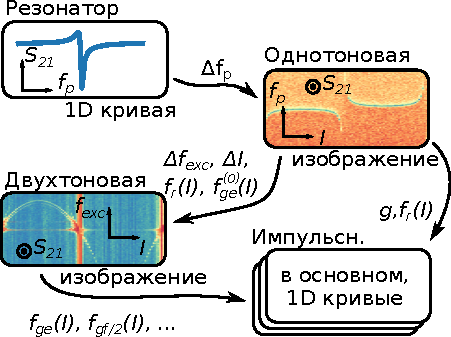
\includegraphics[width=0.5\linewidth]{Pictures/workflow}
	\caption{Схематическое изображение последовательности измерений при экспериментах с образцами квантовой электродинамики цепей со считыванием через резонатор в дисперсионном режиме.}
	\label{fig:workflow}
\end{figure}

В первой части описано экспериментальное оборудование, его ориентировочная стоимость и характеристики, кратко дан принцип работы с приборами через различные программные интерфейсы. Приведен анализ того, какие интерфейсы и форм-факторы лучше использовать в дальнейшем при построении более сложных экспериментов. В качестве примера использования программного кода для управления экспериментом, описана процедура измерения времен когерентности однокубитных образцов и приведены ссылки на оригинальный исходный код, хранящийся в открытом доступе на сайте GitHub \cite{fedorov2021github}.


Во второй части более подробно рассматривается эксперимент по однотоновой микроволновой спектроскопии в архитектуре квантовой электродинамики цепей -- второй шаг на \autoref{fig:workflow}. Для трансмона, связанного с резонатором емкостным образом, частоты на первое и второе возбужденные состояния модели Джейнса-Каммингса будут записываться как 
\begin{align}
f_\pm(I) \equiv f_r(I) = \frac{f_c + f_{ge}(I)}{2} \pm \sqrt{g^2+(f_{ge}(I) - f_c)^2/4},\label{eq:f_r}
\end{align}
где $f_r(I) = f_c$ (частоте резонатора), когда сила связи $g=0$, а $f_{ge}(I)$ -- частота кубитного перехода трансмона -- выражается как
\begin{equation}
f_{ge}(I) = f_{ge}^{max} \left[\cos^2\left(\frac{\pi(I-I_{ss})}{\Pi}\right)+d^2 \sin^2 \left(\frac{\pi(I-I_{ss})}{\Pi}\right)\right]^\frac{1}{4},
\label{eq:tr_spectrum}
\end{equation}
где $I, I_{ss},\ \Pi$ -- это ток, управляющий потоком в СКВИДе трансмона, ток верхней оптимальной точки, период по потоку, а $f_{ge}^\text{max},\ d$ -- частота трансмона в оптимальной точке и асимметрия СКВИДа. Проблема состоит в обнаружении частот $f_{\pm}(I)$ на экспериментальных спектрах, как показано на \autoref{fig:detection}.
	
	
\begin{figure}
	\centering
	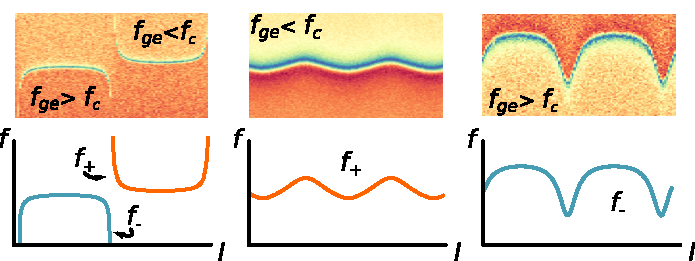
\includegraphics[width=.8\linewidth]{Pictures/detection}
	\caption{Желаемые результаты работы алгоритма при распознавании трех случаев однотоновой спектроскопии}
	\label{fig:detection}
	\end{figure}

В диссертационной работе был предложен и реализован подход на основе метода максимального правдоподобия, позволяющий качественно аппроксимировать экспериментальные данные модельными кривыми. Трудность задача представляет главным образом потому, что модель для случая квазипересечений является разрывной, что делает невозможным прямое применение стандартных методов оптимизации, если заранее неизвестно, какой именно случай из \autoref{fig:detection} будет встречен алгоритмом. Также из-за наличия шума в данных и полном отсутствии информации о начальном приближении требовалось обеспечить дополнительную устойчивость алгоритма путем добавления нескольких промежуточных шагов для аналитического определения периода $\Pi$ и положения оптимальной точки $I_{ss}$. 


\begin{figure}
	\centering
	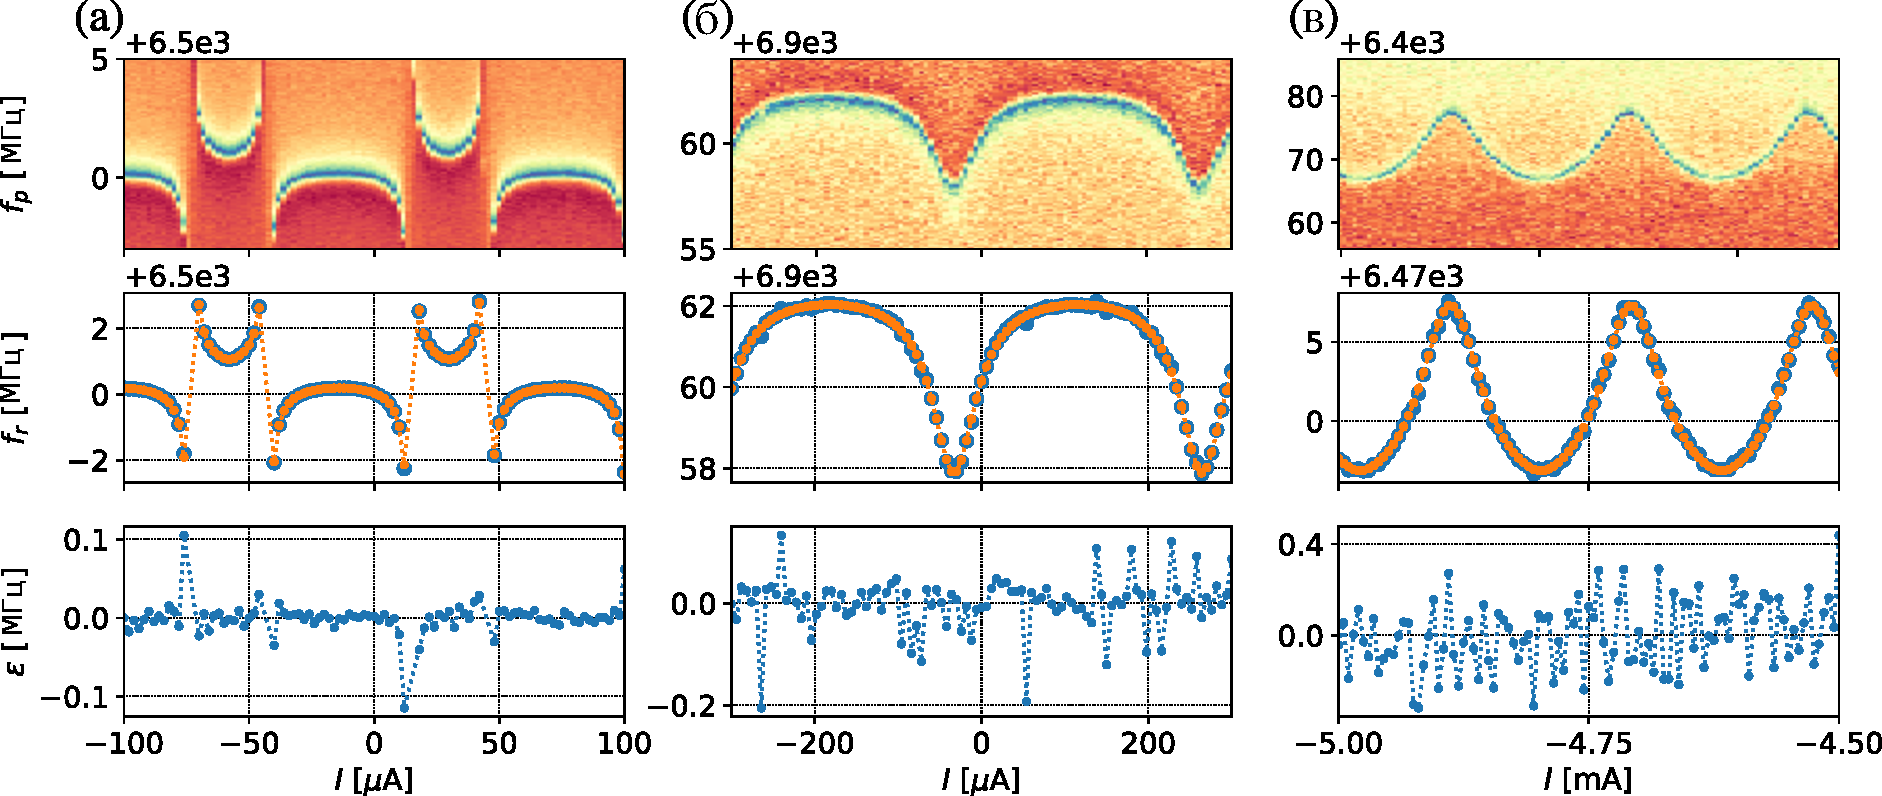
\includegraphics[width=1\linewidth]{Pictures/fit_cases}
	\caption{Результаты работы алгоритма на трех экспериментальных наборах данных, выбранных в качестве примера из нашей базы данных. В верхнем ряду показаны исходные изображения. В среднем ряду построены данные (синие точки) и аппроксимированная модель (соединенные оранжевые точки). В нижнем ряду показаны разности между моделью и данными. Среднеквадратичное отклонение на точку равно: \textbf{(а)} 30 кГц для квазипересечения; \textbf{(б)} 60 кГц для кубита над резонатором; \textbf{(в)} 150 кГц для кубита под резонатором.}
	\label{fig:fitcases}
\end{figure}


\begin{figure}[t]
	\centering
	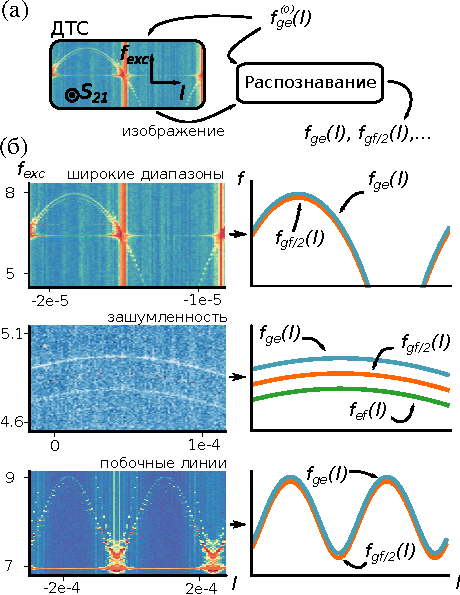
\includegraphics[width=0.6\linewidth]{Pictures/detection_tts}
	\caption{\textbf{(а)} Схематическое изображение принципа анализа результатов ДТС. Приблизительная зависимость частоты кубита $f_{ge}^{(0)}(I)$ от тока служит как для задания области сканирования, так и в качестве начального приближения для алгоритма распознавания. \textbf{(б)} Примеры желаемой работы алгоритма на различных типах данных.}
	\label{fig:detectiontts}
\end{figure}

Результаты работы алгоритма представлены на \autoref{fig:fitcases}. Исходный код программы интегрирован в измерительную библиотеку и также хранится в открытом доступе, файл \foreignlanguage{english}{lib2/fulaut/AnticrossingOracle.py} \cite{fedorov2021github}. Проведены исследование точности опосредованного определения параметров кубита через ММП, проверка устойчивости алгоритма к шуму, профилирование для определения узких мест производительности.


\begin{figure}[t]
	\centering
	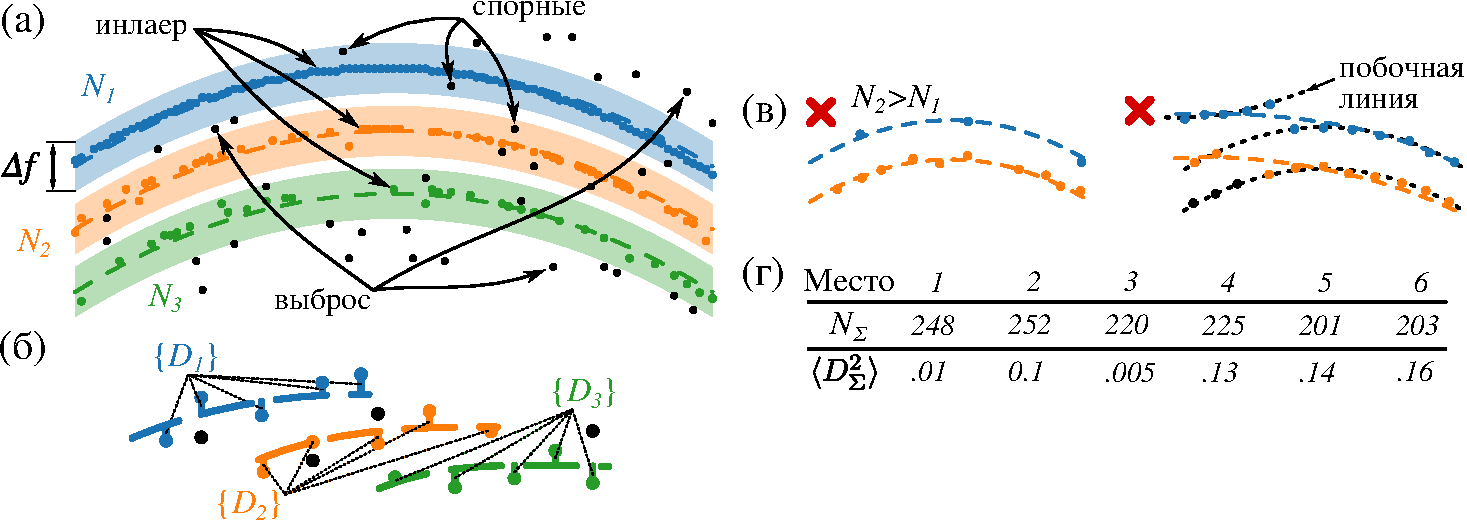
\includegraphics[width=\linewidth]{Pictures/hough_illustration}
	\caption{\textbf{(а)} Вокруг каждой модельной кривой берется симметричный интервал частот шириной $\Delta f$ (выделенные цветом области). Для каждого тока точки вне интервала называются выбросами; из остальных выбирается единственная (ближайшая к модели) точка из интервала -- инлаер, оставшиеся -- спорные. \textbf{(б)} По инлаерам для каждой модели вычисляются среднеквадратичные расстояния $\{D_{1-3}\}$. \textbf{(в)} Дополнительные условия. На основной линии кубита не должно быть меньше точек, чем на какой-либо из побочных; максимизация числа точек не должна происходить за счет ухудшения качества аппроксиммации. \textbf{(г)} Иллюстрация сортировки найденных перебором решений. В первую очередь учитывается число точек, затем среднеквадратичное отклонение данных от модели.}
	\label{fig:houghillustration}
\end{figure}


\begin{figure}
	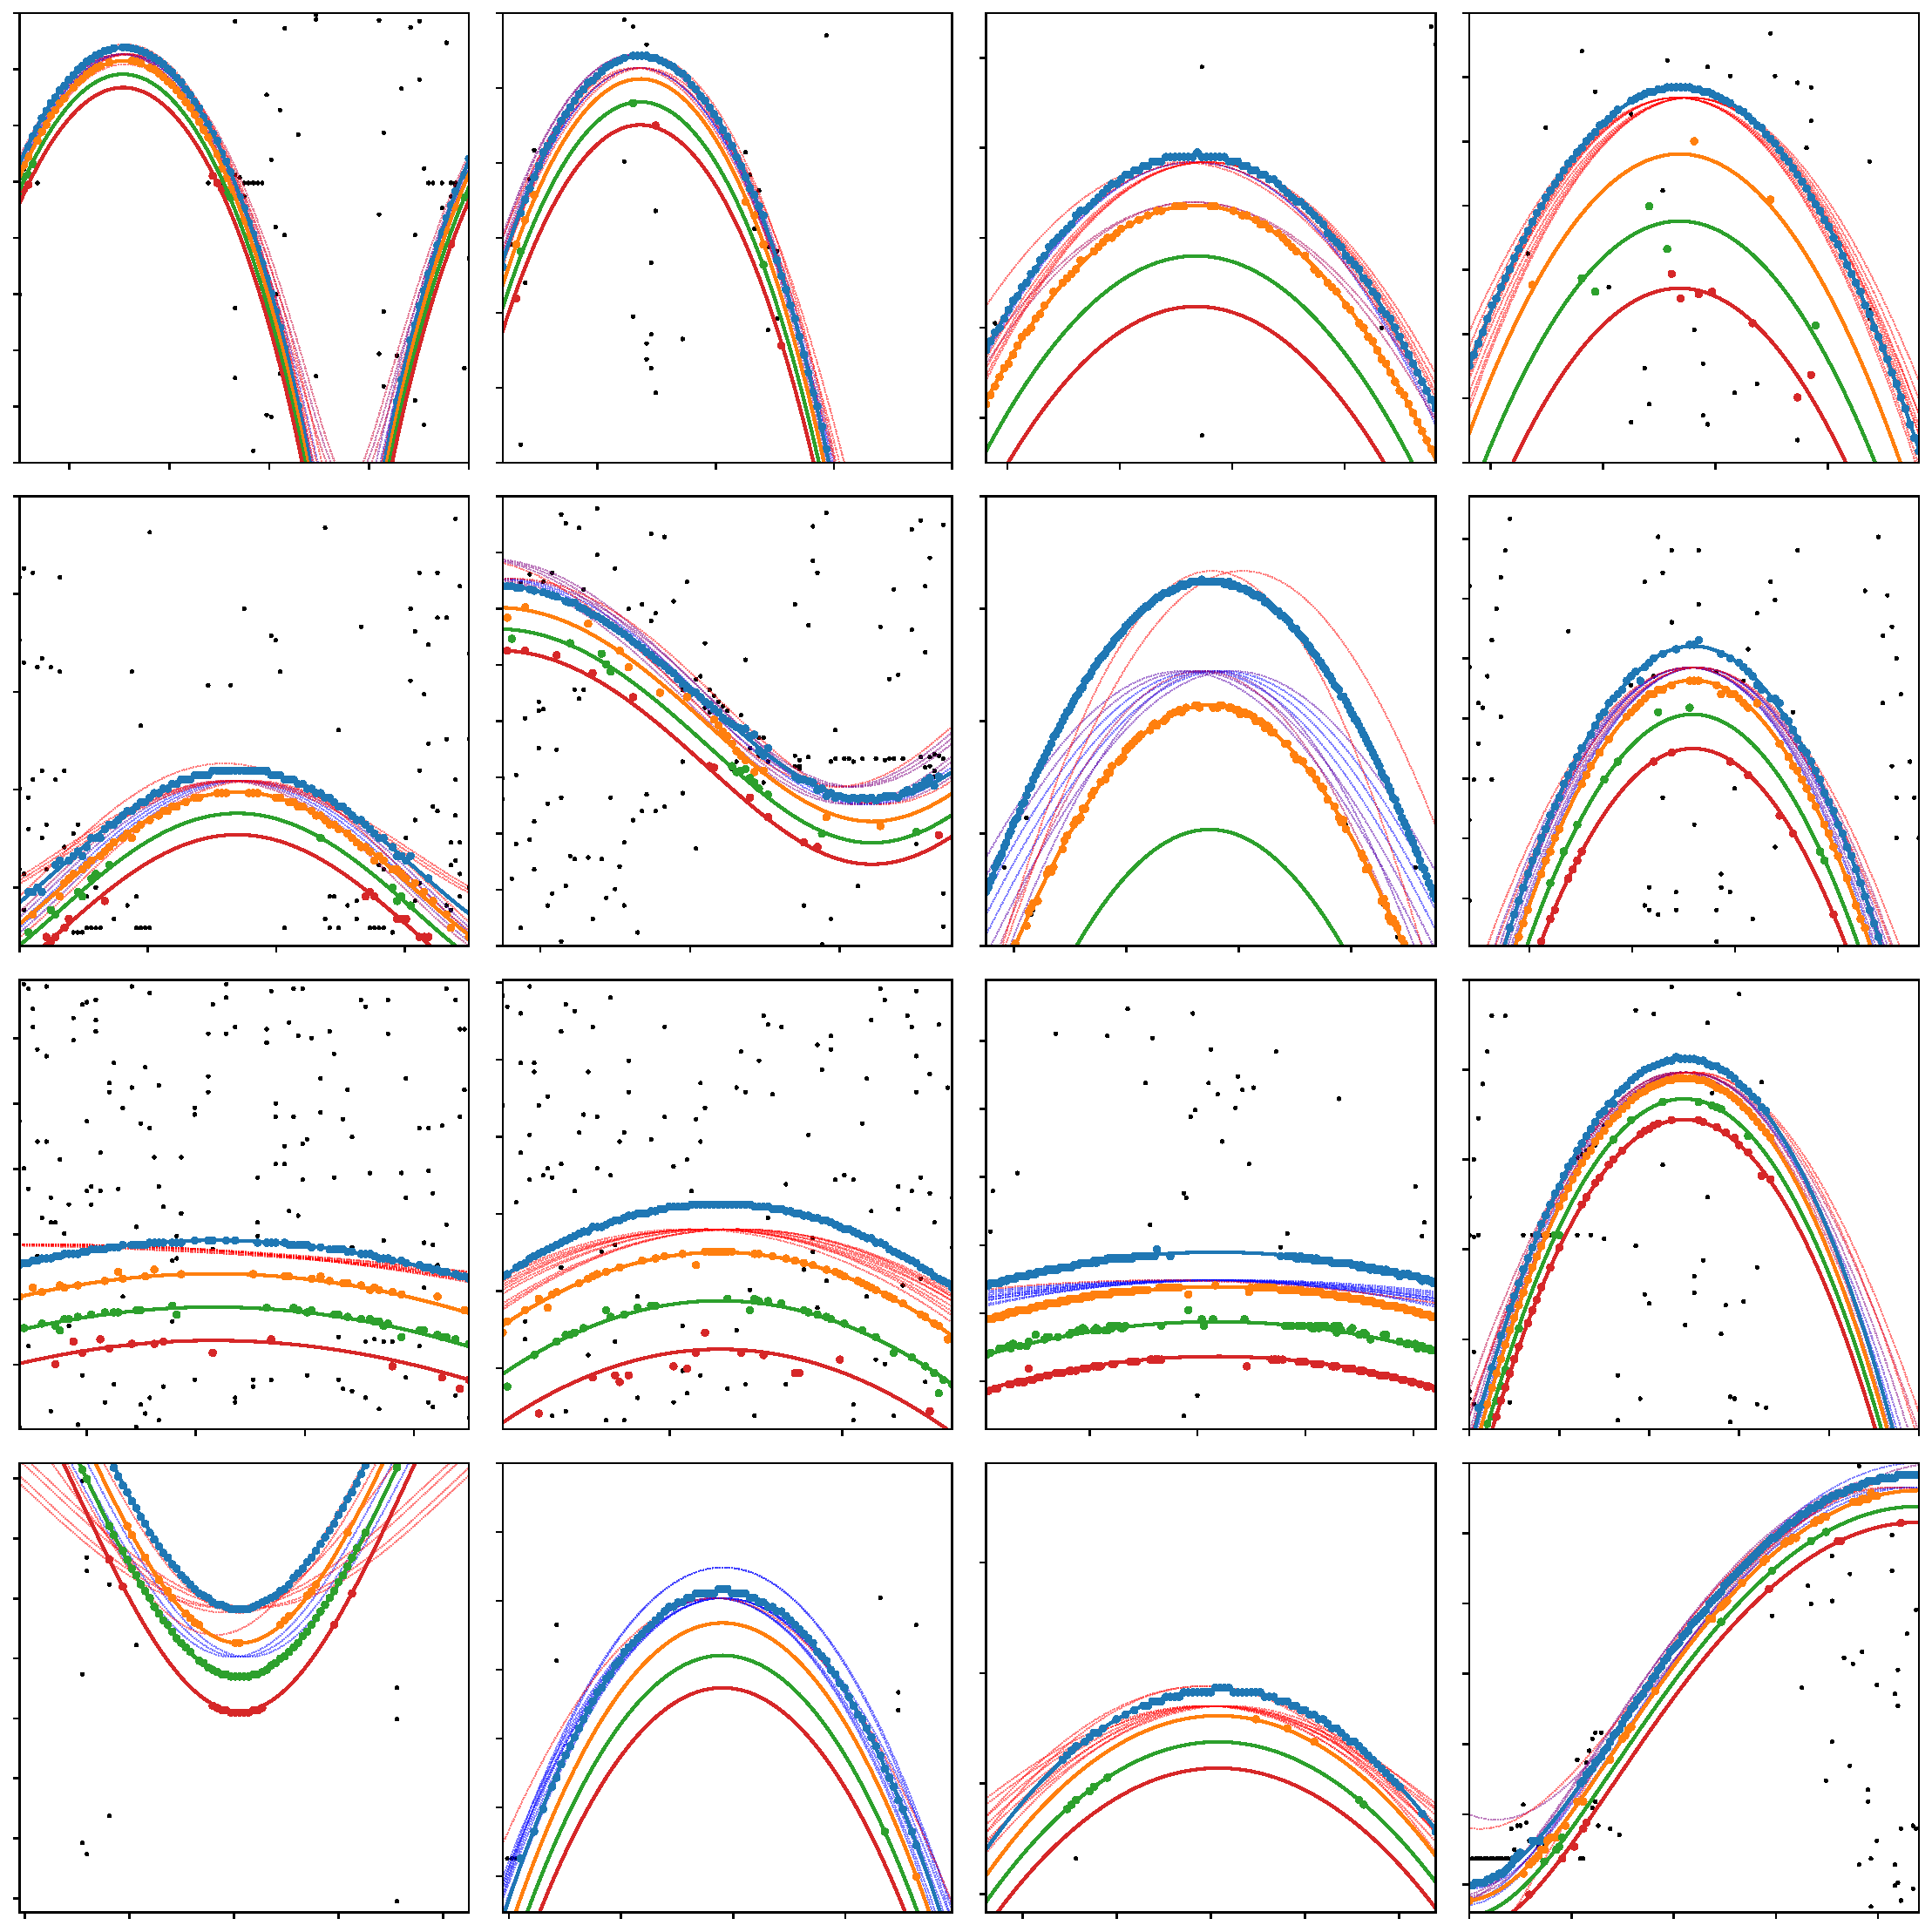
\includegraphics[width=1\linewidth]{Pictures/two_tone_fits}
	\caption{Результаты работы алгоритма на некоторых экспериментальных спектрах. Метапараметры фиксированы, выполнение проводилось в простом цикле по данным и начальным приближениям, полученным при распознавании соответствующих результатов ОТС. Черными точками показаны выбросы, присутствовавшие после предварительной обработки; цветами обозначены аппроксимированные модельные линии и их инлаеры. Тонким пунктиром показаны десять лучших кандидатов, найденных в первом шаге грубой оптимизации.}
	\label{fig:twotonefits}
\end{figure}


В третьей части описывается оригинальная процедура обработки данных двухтоновой спектроскопии. На вход алгоритм должен получать экспериментальный двухтоновый спектр и начальное приближение на основе однотоновых измерений, а на выходе давать параметры спектральных линий трансмона, включая как однофотонные, так и многофотонные переходы, как показано на \autoref{fig:detectiontts} (а). Для того, чтобы алгоритм можно было применять в реальных условиях, он должен был уверенно работать при наличии различных осложняющих факторов, см. \autoref{fig:detectiontts} (б).
	
В диссертационной работе была разработана и программная реализация описанного алгоритма на языке Python, которая также была интегрирована с остальными программами измерительной библиотеки, файл \foreignlanguage{english}{lib2/fulaut/SpectrumOracle.py} \cite{fedorov2021github}. Идея алгоритма для решения поставленной проблемы многомодельной оптимизации была построена на комбинации преобразования Хафа и алгоритма RANSAC. После извлечения положений пиков (локальных максимумов) из двумерных разверток спектроскопии, алгоритму требуется отделить правильные кривые от неизбежно проникающих в силу большого динамического диапазона полезных данных шумовых точек. Схематически предложенная процедура изображена на \autoref{fig:houghillustration}. Для исключения шума производится несколько полных переборов параметров модели, причем для расчета функции потерь берутся только ближайшие к кривой точки из окна определенной ширины по частоте около неё. Таким образом полностью исключается влияние далеких точек на оценку качества аппроксимации. Затем осуществляется сортировка кривых одновременно по количеству точек-инлаеров и среднеквадратичному их отклонению, что возможно сделать, если ранжировать кривые по второму параметру в группах с близкими числами точек (различие по количеству точек не должно, например, превышать 10\% от числа уникальных значений горизонтальной координаты массива точек). Далее осуществляется одновременная численная аппроксимация всех моделей к инлаерам алгоритмом Нельдера-Мида, завершая определение параметров кривой.

Результаты работа алгоритма на 16 примерах экспериментальных данных из собранного в течение выполнения диссертационной работы архива, показаны на \autoref{fig:twotonefits}. Никакие параметры алгоритма не варьировались, за исключением начальных приближений, которые получались для каждого графика из аппроксимации данных соответствующей однотоновой спектроскопии алгоритмом, описанным выше. Как видно, удалось добиться устойчивой работы алгоритма на достаточно широком диапазоне модельных кривых, что дает возможность применять разработанный код в реальных автономно работающих экспериментах.




\paragraph{Третья глава} посвящена экспериментальному исследованию системы из двух связанных кубитов\hyp трансмонов, образующих сверхпроводниковую искусственную молекулу (СИМ), и гибридизацию её состояний с излучением. В литературе, посвященной этой области исследований, представлено большое количество результатов, касающихся исследования двухкубитных систем, однако в рамках выполнения диссертационной работы удалось обнаружить и описать качественно новые спектроскопические проявления эффекта Отлера-Таунса (ЭОТ) в случае, если компоненты молекулы облучаются несимметрично. Подобные эффекты до сих пор не описывались, так как прошлые работы по ЭОТ изучали либо единичные атомы, либо описывали только стандартные спектральные черты эффекта, хорошо известные из квантовой оптики XX века. Если расширить круг поиска и рассмотреть в целом эксперименты по спектроскопии связанных кубитов\hyp трансмонов, то обнаруживается, что и здесь ничего подобного не наблюдали, так как либо использовались сигналы малой мощности, что позволяло различить только основные однофотонные линии , либо для возбуждения переходов на верхние энергетические уровни подавался сигнал с двумя различными частотными компонентами, либо разрешение данных было недостаточным, либо использовались неперестраиваемые по частоте трансмоны. Эксперименты с натуральными молекулами также не фиксировали подобного поведения, что неудивительно, так как трудно исследовать изолированную молекулу, не говоря уже о том, чтобы индивидуально контролировать частоты переходов атомов, из которых она состоит, что физически невозможно.


\begin{figure}[t]
	\centering
	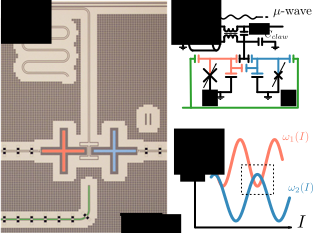
\includegraphics[width=0.7\linewidth]{Pictures/experiment_2}
	\caption{\textbf{(а)} Оптический микрограф устройства (в ложном цвете). Два трансмона (оранжевый, 1 и синий,2) связаны с  копланарным резонатором. Линии управления частотой подходят с боков, снизу подведена микроволновая антенна (зеленый). \textbf{(б)} Эквивалентная электрическая схема. Как перестраиваемые джозефсоновские переходы изображены СКВИДы кубитов\hyp трансмонов, управляемые магнитным полем. \textbf{(c)} Схематический рисунок частот кубитных переходов кубитов\hyp трансмонов $\omega_1 (I)$ и $\omega_2 (I)$ в зависимости от тока внешнего соленоида при правильном выравнивании локальными потоковыми линиями. Пунктиром обведена рабочая область эксперимента.}
	\label{fig:experiment2}
\end{figure}

Оптическая фотография экспериментального образца, разработанного диссертантом и изготовленного на мощностях чистой зоны НОЦ ФМН МГТУ и ВНИИА Духова, изображен на \autoref{fig:experiment2} (а). Гамильтониан связи между трансмонами СИМ состоит из двух компонент: прямое электрическое взаимодействие и опосредованное дисперсионное через квантовую шину, которая служит также и для совмещенного дисперсионного считывания, как показано на \autoref{fig:experiment2} (б). Излучение подается через антенну (отдельный копланарный волновод) сразу на обе подсистемы. В эксперименте проводится спектроскопия с высоким разрешением в области, показанной пунктиром на \autoref{fig:experiment2} (в).


\begin{figure}
	
	\centering
	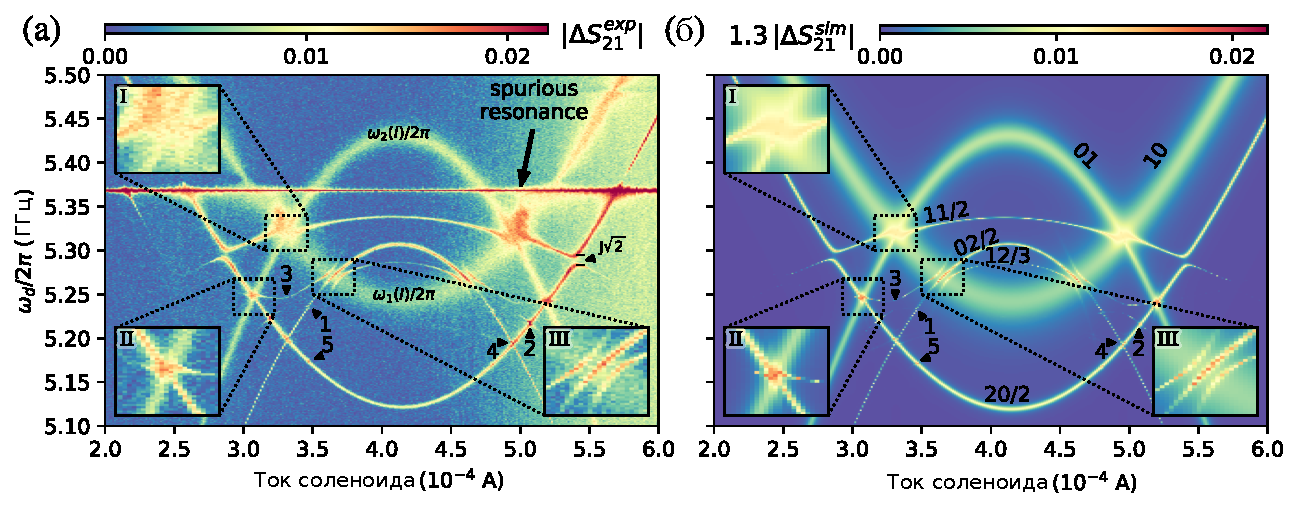
\includegraphics[width=\linewidth]{main_picture}
	
	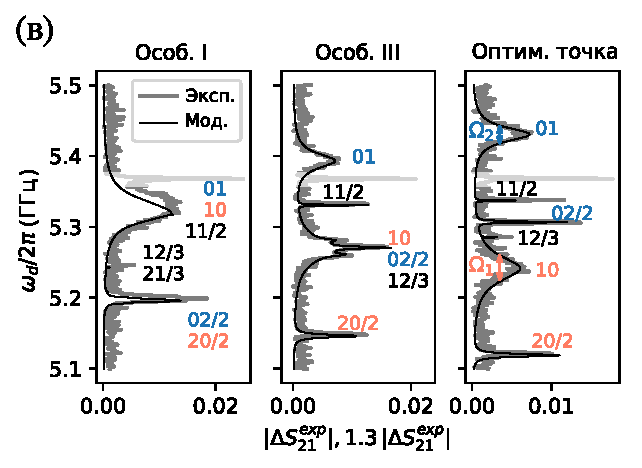
\includegraphics[width=.495\linewidth]{main_picture_slices}
	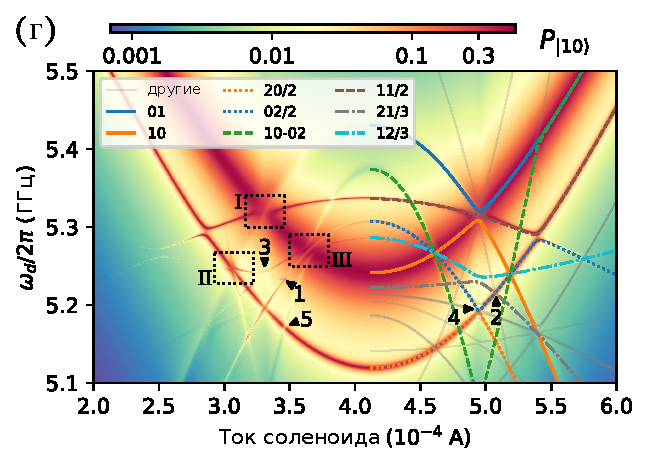
\includegraphics[width=.495\linewidth]{stationary}
	\caption{\textbf{(a)} 
		Данные ДТС. Цветом показан модуль отклонения $|\Delta S^{exp}_{21}| (I, \omega_d)$ комплексного коэффициента пропускания от значения в левом нижнем углу графика. 
		Трансмоны выровнены как на 
		\autoref{fig:experiment2}~(в) и их спектральные линии формируют симметричную картину. Три эффекта, не предсказываемые невозмущенной моделью, показаны во вставках I, II и III; остальные особенности, воспроизводящиеся полной численной моделью, пронумерованы арабскими цифрами. \textbf{(б)} Результаты численного расчета. Рассчитанное значение $|\Delta S^{sim}_{21}| (I, \omega_d)$ искусственно увеличено в 1.3 раза для достижения количественного совпадения с экспериментом.
		\textbf{(в)} Срезы (а) and (б) при нескольких значениях тока соленоида: 0.333 мA (особенность I), 0.365 мA (особенность III), 0.411 мA 
		(оптимальная точка); 
		экспериментальные данные показаны серым, счет черным цветом. \textbf{(г)} Рассчитанная заселенность  
		уровня $\ket{10}$ в зависимости от $I$ and $\omega_d$. Кривыми показаны частоты разнообразных переходов, вычисленные из невозмущенного гамильтониана. Линии, аппроксимирующие основные переходы, подписаны на графике в таком порядке, как они расположены в окрестности оптимальной точки. Под отметкой ``другие'' помещены все остальные переходы системы, попадающие в диапазон частот графика.}
	\label{fig:two-tone}
\end{figure}

Результаты спектроскопии представлены на \autoref{fig:two-tone} (а). Главные особенности спектра, обозначенные римскими цифрами I, II, III, обнаружены и описаны впервые и являются следствием сложной модификации ЭОТ, когда монохроматическое излучение оказывается одновременно как зондирующим, так и одевающим сигналом. Помимо этих особенностей, в диссертации подробно описаны и вторичные, менее заметные черты, обозначенные на графике арабскими цифрами.

Проводилось также численное моделирование на основе решения основного уравнения для эволюции подсистемы для установившейся матрицы плотности, которая затем подставлялась в выражение для вычисления среднего оператора совмещенного считывания. Было получено в целом хорошее совпадение данных с экспериментом, за исключением проблем с воспроизведением высот и ширин некоторых многофотонных пиков и общего увеличения всех сигналов примерно на 30\% по сравнению с предсказанным [\autoref{fig:two-tone} (б, в)]. На \autoref{fig:two-tone} (г) показана населенность состояния $\ket{10}$, в котором однократно возбужден первый трансмон. Видно, что особенность III образуется пересечением переходов 10, 02/2 (двухфотонным), 12/3 и 10-02, то есть выполнением сложного резонансного условия между однофотонными и многофотонными переходами.
	

\begin{figure}[t]
	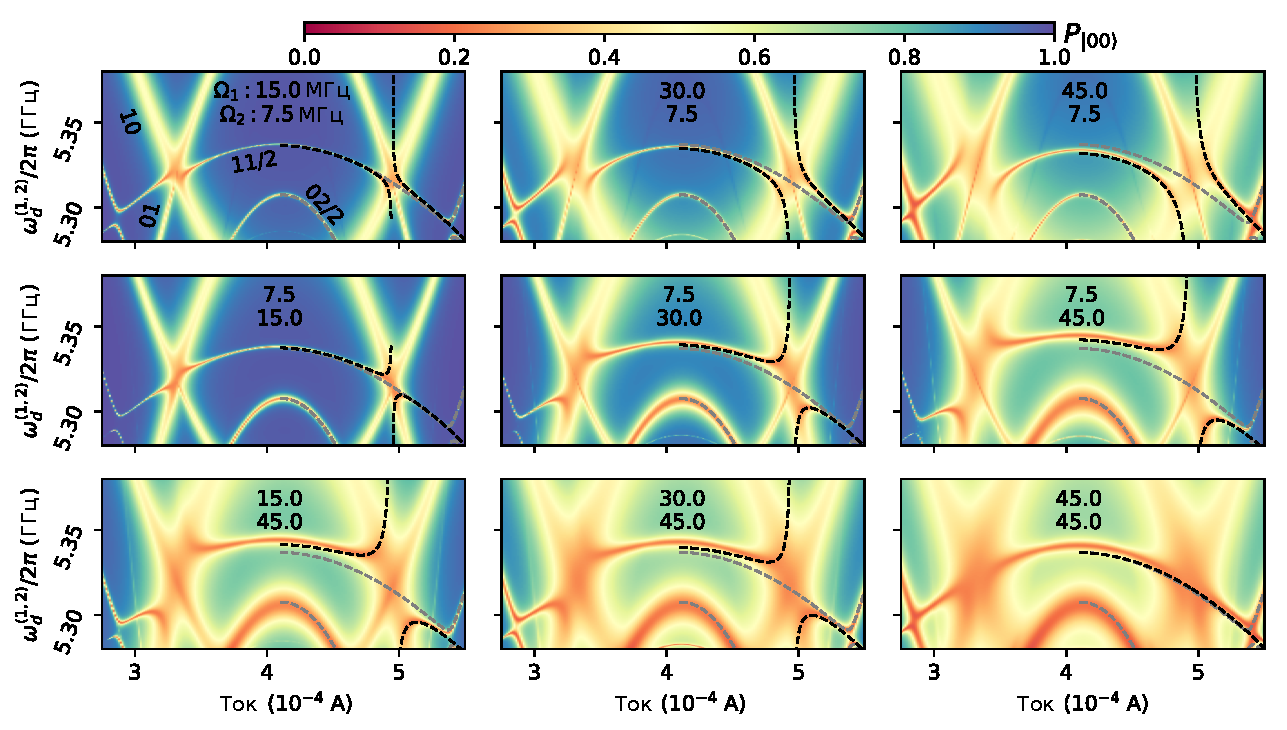
\includegraphics[width=1\linewidth]{Pictures/topological_splittings}
	\caption{Численное моделирование зависимости особенности I от мощности. Цветом показана заселенность основного состояния в установившемся состоянии, когда трансмоны облучаются на одной частоте, но с разными интенсивностями $\Omega_{1,2}$. В верхнем (среднем) ряду, 
		$\Omega_{1(2)}$ увеличивается, в то время как
		$\Omega_{2(1)} = \text{const},\ \Omega_{2(1)} < 
		\Omega_{1(2)}$; две топологически отличные схемы расщепления возникают в зависимости от того, на каком из кубитов\hyp трансмонов интенсивность излучения больше. В нижнем ряду показано, как расщепления исчезают, если более слабое возмущение доводится по уровню до более сильного. Серые штриховые линии показывают невозмущенное решение, а черным показаны модельные кривые.}
	\label{fig:topologicalsplittings}
\end{figure}

Были построены самосогласованные аналитические модели, описывающие форму наблюдаемых квазипересечений с учетом их зависимости от интенсивности излучения. Например, для особенности III полученная аналитическая формула выглядит следующим образом:
\begin{equation}
\omega_d^{(III, \pm)} = \frac{2 \alpha_2}{3} + \frac{4 \omega_{2}}{3} - \frac{\omega_{1}}{3} \pm \frac{\sqrt{3 \Omega_{1}^{2} + \left( \alpha_2 + 2 (\omega_{2} - \omega_{1})\right)^{2}}}{3}.
\label{eq:splitting_model}
\end{equation}

Удалось описать также и поведение системы в области I, где однофотонные переходы одевают кубитные переходы обоих кубитов\hyp трансмонов одновременно. Экспериментально эффект слабо различим из-за фиксированного и близкого к единице отношения частот Раби, $\Omega_1/\Omega_2 \approx 2$ (эффект пропадает в случае $\Omega_1 = \Omega_2$), однако в численном моделировании для произвольных $\Omega_{1,2}$ можно получить ярко выраженные квазипересечения, показанные на \autoref{fig:topologicalsplittings}. Для этого режима самосогласованным методом получено универсальное выражение, описывающее поведение частоты двухфотонного перехода 11/2, зондирующего получающуюся систему уровней:
\begin{equation}
\omega_d^I = \frac{\omega_{1} + \omega_{2}}{2} + \frac{\Omega_{1}^{2} - \Omega_{2}^{2}}{ 2\left(\omega_{1} - \omega_{2}\right)}
\label{eq:topo_comm}
\end{equation}
Выражение расходится в области равенства частот кубитов, и поэтому может применяться в области $|\omega_1 - \omega_2| \geq J$.

\paragraph{Четвертая глава} посвящена экспериментальному и теоретическому исследованию прохождения излучения через цепочку из пяти кубитов\hyp трансмонов, подключенную к двум полубесконечным волноводам на своих краях. Предложенное устройство демонстрирует возможность проведения экспериментов с проектированием динамики Флоке, когда вместо дискретных квантовых операций на систему подается непрерывное излучение на наборе частот, что делает невозможным применение переход во вращающийся базис и решение задачи эволюции через матричную экспоненту. Нахождение волновой функции системы в таком режиме возможно только путем полного решения дифференциального уравнения Шредингера и представляет большую трудность по сравнению с классическим воспроизведением результатов обычного квантового алгоритма через последовательное умножение матриц большой размерности. 
 
\begin{figure}[t]
	\centering
	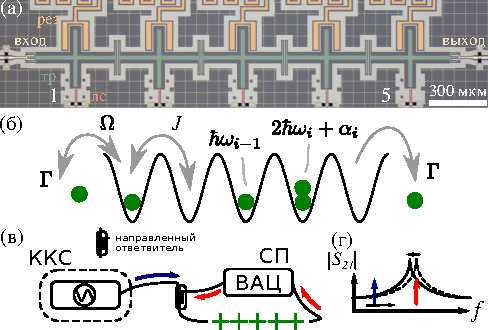
\includegraphics[width=0.8\linewidth]{Pictures/scheme_bh}
	\caption{\textbf{(а)} Оптическое изображение устройства (в ложном цвете). Входной и выходной волноводы (бежевый) сильно связаны с трансмонами (зеленый) на краях цепочки. Трансмоны могут считываться дисперсионно вспомогательными резонаторами (оранжевый) и перестраиваться по частоте линиями смещения (красный). \textbf{(б)} Модель, отображаемая на устройство -- решетка Б-Х с пятью ячейками. Бозоны поступают справа из входящего возбуждения амплитуды $\Omega$ и утекают, главным образом, на краях со скоростью $\Gamma$. Энергия $i$-го локализованного бозона равна $\hbar\omega_i$, добавление еще одного бозона в ту же ячейку требует энергии $\hbar \alpha_i<0$. Бозоны также могут туннелировать между соседними ячейками со скоростью $J$. \textbf{(в)} Качественное изображение измерительной установки: спектроскопия пропускания (СП) делается при помощи векторного анализатора цепей (ВАЦ), измеряющего комплексное пропускание $S_{21}$. Кросс-керровская спектроскопия (ККС) требует добавления отдельного микроволнового генератора, подключаемого через направленный ответвитель. \textbf{(г)} ККС производится путем развертывания частоты дополнительного генератора (синяя стрелка) и наблюдения изменений в пропускании в области одного из резонансов анализатором цепей (красная стрелка).}
	\label{fig:schemebh}
\end{figure}


Экспериментальный образец представлен на \autoref{fig:schemebh} (а). Для проведения экспериментов использовались пять емкостно связанных и перестраиваемых по частоте иксмонов (образец был спроектирован диссертантом и изготовлен в НОЦ ФМН МГТУ и ВНИИА Духова). Сильная связь с двумя открытыми одномерными пространствами обеспечивается при помощи крупных встречно-штыревых конденсаторов, размещенных на концах копланарных волноводов, и позволяет измерять электромагнитное пропускание через структуру. На \autoref{fig:schemebh} (б) приведена иллюстрация физической модели, которая отображается на устройство; соответствующий гамильтониан с учетом когерентной накачки может быть записан как
\begin{equation}
\begin{aligned}
\hat H/\hbar &= \sum_{i=1}^5\left[ (\omega_i - \omega_d) \hat b^\dag_i \hat b_i + \frac{1}{2} \alpha_i \hat b_i^\dag \hat b_i (\hat b^\dag_i \hat b_i - 1)\right]\\
&+J\sum_{i=1}^4 \left[\hat b^\dag_{i+1} \hat b_i + \hat b_{i+1} \hat b_i^\dag\right]+\frac{\Omega}{2}(\hat b_1^\dag + \hat b_1),
\end{aligned}\label{eq:bose-hubbard}
\end{equation} 
где $\hat b_i$, $\hbar \omega_i$ и $\hbar \alpha_i$ -- это, соответственно, оператор уничтожения, энергия одиночного локализованного бозона и энергия взаимодействия бозонов  для $i$-ой ячейки; туннелирование между ячейками происходит со скоростью $J$, а циклическая частота накачки равна $\omega_d$ . Диссипативные процессы учитывались при помощи уравнения Лиувилля с линдбладовскими сверхоператорами на основе операторов коллапса, описывающих релаксацию и чистую дефазировку на каждой ячейке со скоростями $\gamma_i$ и $\gamma_{\phi}^{(i)}$. Сильная связи с линией подразумевает, что $\gamma_1 \approx \gamma_5 = \Gamma$ являются основным источником декогеренции. Если $\omega_i = \omega$, $\alpha_i = \alpha$, то восстанавливается стандартный вид гамильтониана модели Б-Х.

На \autoref{fig:schemebh} (в) схематически изображена экспериментальная установка для измерения свойств образца. Мы измеряем комплексный коэффициент матрицы рассеяния для пропускания через двухпортовое устройство $S_{21}$ при помощи векторного анализатора цепей (спектроскопия пропускания, СП) и, дополнительно используя микроволновый генератор, осуществляем кросс-керровскую спектроскопию (ККС) системы; в обоих случаях используются непрерывные микроволновые сигналы и исследуется установившееся поведение системы. Для получения теоретического предсказания параметра $S_{21}$ использовался формализм квантовой теории отклика.
	
Результаты спектроскопии пропускания показаны на \autoref{fig:dts-cks} (а). Чтобы продемонстрировать структуру собственных состояний и точно извлечь $\omega_i$ и $J$, мы смещаем один из кубитов\hyp трансмонов по частоте вокруг точки вырождения, в то время как остальные зафиксированы на $4.05$ ГГц. В левой колонке \autoref{fig:dts-cks} смещается потоком первый трансмон, а в правой -- средний. Как можно видеть, первый взаимодействует со всеми коллективными состояниями, а третий только с нечетными; по модельным кривым можно понять, что такое поведение полностью предсказывается гамильтонианом \eqref{eq:bose-hubbard} без накачки. С помощью численной аппроксимации мы определяем, что скорость туннелирования $J/2\pi\approx 41$ МГц.
	
	\begin{figure}[t]
		\centering
		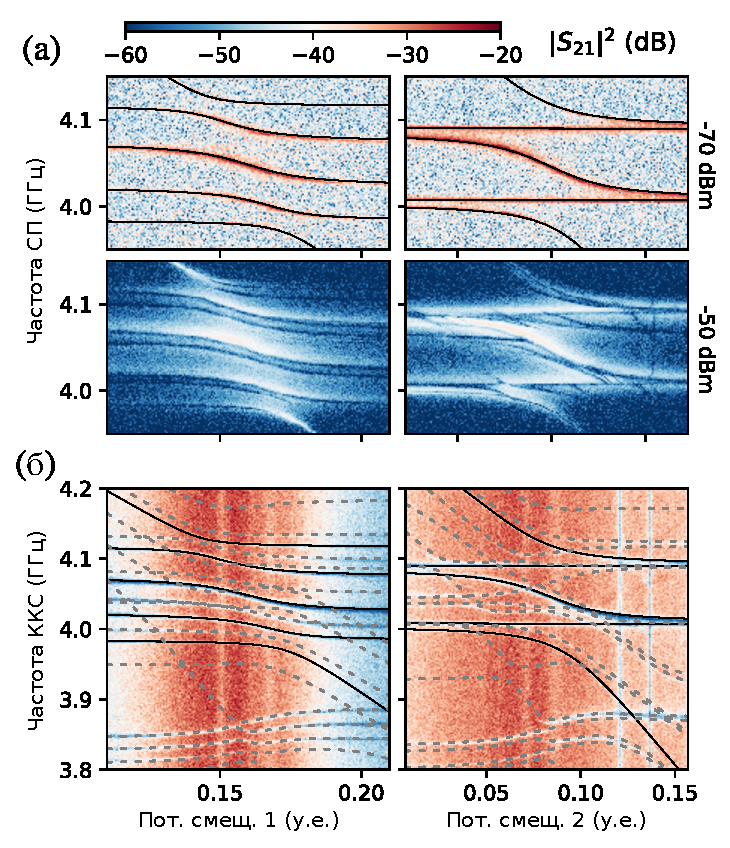
\includegraphics[width=0.6\linewidth]{Pictures/DTS-CKS}
		\caption{\textbf{(а)} Данные ПС цепочки в зависимости от потокового смещения одного из кубитов\hyp трансмонов. $S_{21}$ включает аттенюацию и усиление в измерительном тракте, мощность ВАЦ показана справа. В верхнем ряду черные сплошные линии показывают предсказание Ур. \eqref{eq:bose-hubbard} для частот нижних пяти переходов при $J/2\pi = 41$ МГц, $\omega_i/2\pi \approx$ 4.05 ГГц, $\Omega=0$. \textbf{(б)} ККС на третьей по порядку моде, показывающая зарождающуюся зонную структуру системы. Прерывистыми линиями показаны предсказания модели для частот чисто квантовых переходов.}
		\label{fig:dts-cks}
	\end{figure}

При увеличении мощности падающего сигнала, на пропускании наблюдается эффект фотонной блокады, заключающийся в спадании пропускания пропорционально приложенной мощности. Подобные эффекты часто наблюдаются при исследовании одиночных сверхпроводниковых кубитов, связанных с микроволновой линией . В нижнем ряду \autoref{fig:dts-cks} (а) мы наблюдаем также и признаки возбуждения многочастичных состояний системы, которые уже не имеют классических аналогий. Изменения в поведении системы при увеличении мощности мы поэтому называем переходом от классического к квантовому режиму. Остающиеся параметры $\alpha_i$ Ур. \eqref{eq:bose-hubbard} можно определить путем аппроксимации данных ККС, результаты которой показаны на \autoref{fig:dts-cks} (б) для тех же конфигураций частот кубитов\hyp трансмонов, что и на фрагменте (а).

Для более подробного изучения энергетической структуры и неравновесной динамики системы при переходе к неклассическому режиму, проводился еще один эксперимент по спектроскопии пропускания с фиксированной вырожденной конфигурацией кубитов\hyp трансмонов на частоте $\omega/2\pi = 3.9$ ГГц.
\begin{figure}[h!]
	\includegraphics[width=1\linewidth]{Pictures/ckt}
	
	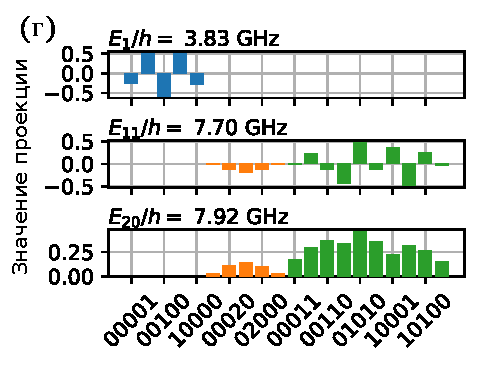
\includegraphics[width=.328\linewidth]{Pictures/eigenstates1}
	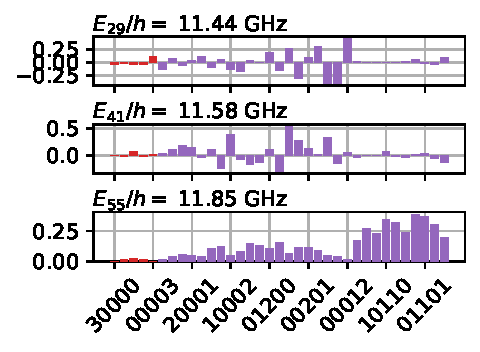
\includegraphics[width=.328\linewidth]{Pictures/eigenstates2}
	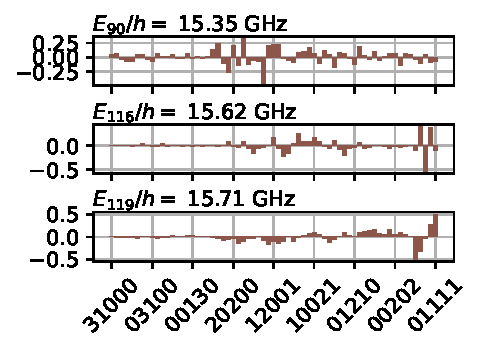
\includegraphics[width=.328\linewidth]{Pictures/eigenstates3}
	\caption{\textbf{(а)} Аналитическое решение для $S_{21}$ в линейном режиме (черные сплошные кривые) аппроксимированные к данным для малой мощности (точки), c нормировкой. \textbf{(б)} Экспериментальные и численные данные для $|S_{21}|$ для различных мощностей накачки. Мощность накачки откалибрована для совпадения с параметром $\Omega$ численного расчета. Штрихами показаны частоты многофотонных переходов, полученных из численно рассчитанных собственных уровней энергии, изображенных на (в). \textbf{(в)} Энергетическая структура системы со взаимодействием и без него при значениях параметров, полученных из численной аппроксимации; учитывается максимум три возбуждения на ячейку и четыре на всю цепочку; $E_n$ -- энергия $n$-го состояния, $E_0 =0$. \textbf{(г)} Некоторые относящиеся к экспериментально наблюдаемым переходам состояния модели, согласно численному расчету, в проекции на невозмущенный базис (цвета из фрагмента (в)). ``Врожденная'' случайность в коэффициентах разложения высокоэнергетических состояний обуславливает произвольность в распределении уровней энергии.}
	\label{fig:ckt}
\end{figure}
В линейном режиме мы оцениваем потери из-за связи с микроволновыми линиями на крайних трансмонах и собственную диссипацию на внутренних путем численной аппроксимации комплексного пропускания в зависимости от частоты линейной моделью, полученной из уравнений Ланжевена и изображенной на \autoref{fig:ckt} (а). При увеличении мощности сигнала пики нормальных колебаний постепенно насыщаются и уширяются за счет фотонной блокады; одновременно с этим возникают новые линии с существенно подавленным пропусканием и связанные с отражением от цепочки в результате многофотонных переходов в многочастичные состояния. Экспериментальные данные хорошо согласуются с численным расчетом для установившегося режима для модели Бозе-Хаббарда с пятью трехуровневыми ячейками, результаты которого показаны на \autoref{fig:ckt} (б). На \autoref{fig:ckt} (в) показаны проекции некоторых из них на базис факторизованных состояний при $J=0$. Состояние $\ket{1}$ идентично по структуре классической симметричной низкочастотной нормальной моде колебаний. Состояния $\ket{11}$ и $\ket{20}$ находятся на краях зеленой подзоны двухфотонного подпространства и являются суперпозициями гораздо большего размера. Уже для этих состояний можно заметить раскрывающуюся случайность в коэффициентах разложения, которая становится все более и более выраженной с ростом энергии так же, как и в случае с энергетическими уровнями. Никакой симметрии или хотя бы какой-то структуры не наблюдается для высших энергетических состояний, за исключением дырочного подпространства с четырьмя возбуждениями, двойственного однофотонному подпространству (см. правую часть графиков для $\ket{116}$, $\ket{119}$).

\begin{figure}
	\centering
	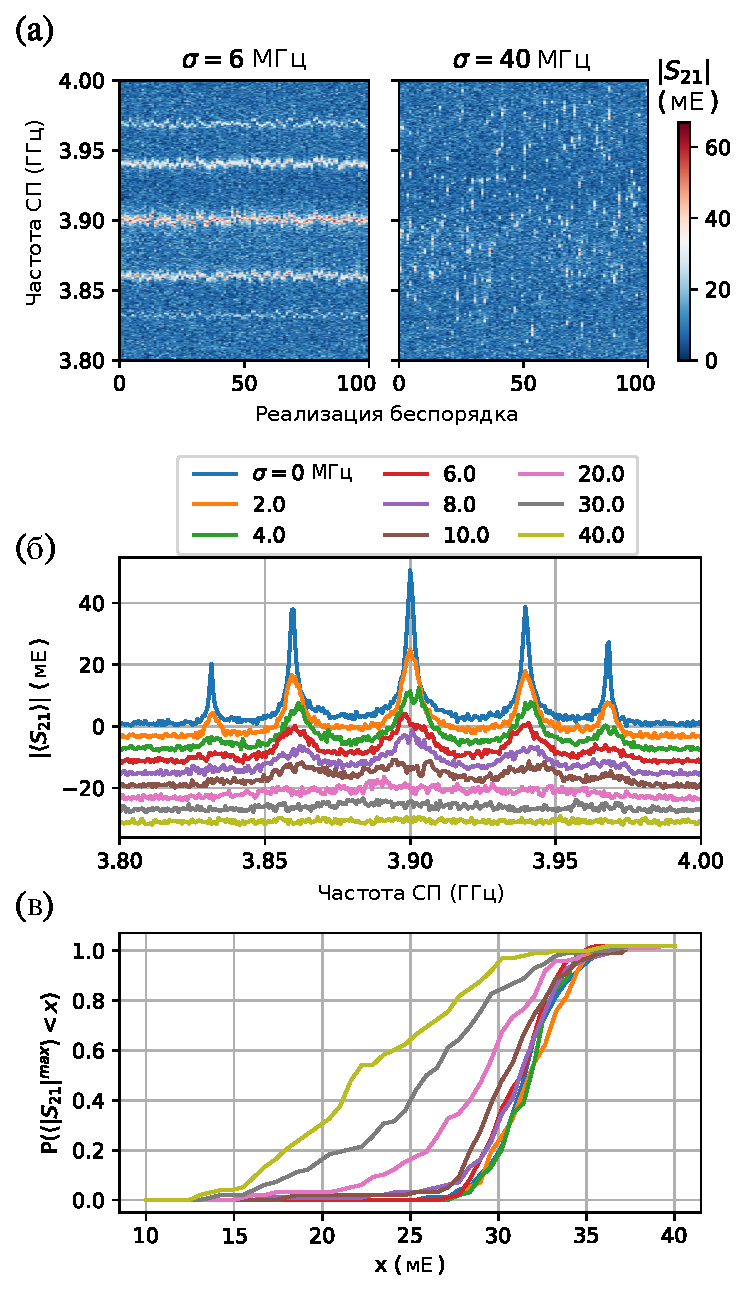
\includegraphics[width=0.6\linewidth]{Pictures/mbl}
	\caption{\textbf{(а)} Сырые данные пропускания для $\sigma = 6, 40$ МГц и 100 реализаций беспорядка; модуль $S_{12}$ показан цветом. \textbf{(б)} Локализация и прекращение транспорта с увеличением беспорядка. Каждая кривая показывает абсолютную величину усредненного по заданному экспериментально нормальному распределению пропускания с выбранным $\sigma$, показанным в легенде. Каждая следующая кривая смещена вниз на 4 мЕ для наглядности. \textbf{(в)} Функции распределения для величины самого яркого из пиков $\langle |S_{21}^{\text{max}}\rangle$ для каждой реализации, построенные для значений $\sigma$ из (б).}
	\label{fig:mbl}
\end{figure}
Наконец, изучалась многочастичная локализация в системе, вызванная беспорядком. Чтобы выяснить, как локализация меняет транспортные свойства системы, мы вносим контролируемый беспорядок в частоты кубитов\hyp трансмонов, распределяя их случайно вокруг точки вырождения в эксперименте, похожем на ранее проводившиеся другими группами численные опыты. Для всех кубитов\hyp трансмонов выбирается определенное среднеквадратичное отклонение $\sigma$, а затем каждому выставляется частота $\omega + \delta \omega$, где $\delta \omega \in \mathbb{N}(0, 2\pi \sigma)$ и $\omega/2\pi = 3.9$ ГГц. Затем записывается экспериментальное пропускание и процесс повторяется 100 раз (количество здесь было ограничено главным образом временем измерения и стабильностью системы). На \autoref{fig:mbl} (а) мы показываем два примера сырых данных до усреднения. Для меньших $\sigma$ собственные состояния мало чувствительны к беспорядку и сохраняют свою структуру, но при $\sigma \approx J/2\pi$ моды практически распадаются. Усредненные кривые показаны на \autoref{fig:mbl} (б) для нескольких значений $\sigma$: при достижения разбросом энергий ячеек скорости туннелирования между ними, усредненное пропускание исчезает. Таким образом, локализация проявляется в прекращении нелокального транспорта -- одиночные фотоны, в среднем, не могут протуннелировать до противоположного конца цепочки. Это поведение напоминает переход сверхпроводник-изолятор, для описания которого изначально и предлагалось использовать модель Бозе-Хаббарда. Так как пропускание пропадает только в среднем, а в каждом отдельном случае в силу случайности пики пропускания могут появляться даже при самом большом значении $\sigma$, мы строим также величину видности пиков, которую мы (достаточно произвольно) определяем как среднее по 10 точкам вокруг самого высокого значения пропускания. Однако, как видно на \autoref{fig:mbl} (в) распределение этой величины испытывает качественное изменение при приближении $\sigma$ к $J/2\pi$.

\paragraph{В заключении} подводятся итоги выполненных в диссертационной работе исследований и полученных результатов.
	
\section*{Основные результаты диссертационной работы}

\begin{enumerate}
	\item \textbf{Разработан программный код для автоматизации экспериментов со сверхпроводниковыми кубитами, создана система для автоматической калибровки физических параметров образцов на основе алгоритмов компьютерного зрения} \citeA{fedorov2019automated}. Впервые предложен алгоритм на основе метода максимального правдоподобия для оценки параметров кубита-трансмона, связанного с резонатором, в архитектуре квантовой электродинамики цепей из данных однотоновой спектроскопии (ОТС) векторным анализатором цепей. Показано, что предложенный метод позволяет аппроксимировать любую из трех возможных зависимостей резонансной частоты от магнитного потока и устойчив к шуму, в то же время обладая достаточно высокой производительностью и точностью для применения на практике. Алгоритм может использоваться и в других целях: например, для установления матрицы индуктивности и определения перекрестных взаимодействий основываясь исключительно на данных ОТС. Также преложен оптимизационный метод автоматической многомодельной обработки данных двухтоновой спектроскопии (ДТС) с чертами преобразования Хафа и алгоритма RANSAC, способный устойчиво работать в условиях количественного преобладания шумовых точек и наличия паразитных спектральных линий, отличающихся по форме от искомых. Разработанные библиотеки использовались в работах \citeA{Besedin2018880, Kalacheva2020, fedorov2020light, fedorov2021photon}.

\item \textbf{Экспериментально обнаружены и исследованы теоретически эффекты гибридизации излучения с двухатомной искусственной молекулой на основе связанных кубитов\hyp трансмонов} \citeA{fedorov2020light}. Система подвергалась интенсивному воздействию СВЧ-сигнала, так что возможно было наблюдать значительное количество многофотонных переходов, отражающих структуру уровней композитной системы за пределами двухкубитного базиса. Благодаря высокой когерентности системы среди таких переходов удалось обнаружить отличия от предсказаний стационарного уравнения Шредингера без учета излучения, заключавшихся в образовании новых квазипересечений, размер которых оказался зависящим от мощности сигнала, т.е. от Раби-частоты. Эффект был идентифицирован как ранее не наблюдавшаяся разновидность эффекта Отлера-Таунса (ЭОТ), в котором разделение сигналов происходит не за счет разности их частот, но за счет того, на какое гильбертово подпространство действуют соответствующие им операторы возмущения и какого порядка процессы ими вызываются. Так как в такой конфигурации используется монохроматический, для наблюдения эффекта требуется выполнение сложного резонансного условия в структуре уровней и одновременного совмещения не-резонансного расщепления одетых состояний одного кубита с многофотонным перехода по состояниям другого. Были предложены самосогласованные модели, точно предсказывающие положение триплетов для всех наблюдавшихся квазипересечений.

\item \textbf{Экспериментально исследована цепочка из пяти кубитов\hyp трансмонов в режиме моделирования диссипативной системы Бозе-Хаббарда с накачкой} \citeA{fedorov2021photon}. Для этого к ее противоположным концам подключались два СВЧ-волновода, в один из которых подавался сигнал переменной мощности с одного входа векторного анализатора, а другой был подключен через малошумящий усилитель к другому его входу. Было экспериментально показано, что в линейном режиме при малой мощности накачки система ведет себя в полном согласии с классической теорией нормальных колебаний для пяти связанных осцилляторов в духе принципе соответствия: волновые функции такой системы оказываются дуальны векторам нормальных мод и такими же свойствами обладает и спектр пропускания. Однако при повышении мощности сигнала наблюдается эффект фотонной блокады и обнаруживаются переходы на уже строго квантовомеханические многочастичные состояния, не имеющие классического аналога. Далее, система подвергалась введению в частоты кубитов беспорядка, имитирующего наличие потенциальных барьеров между ячейками. Было обнаружено соответствие поведения пропускания через систему с ранее исследованными эффектами многочастичной локализации: в среднем пропускание прекращается, когда разброс частот оказывается порядка скорости туннелирования одиночных возбуждений между трансмонами. Таким образом было подтверждено, что композитная квантовая система, работающая в режиме сильной связи с континуумом мод, может сохранять свои квантовые свойства, что явственно проявляется в излучаемом ею свете. Этот эксперимент открывает новые пути для исследований в области разработки алгоритмов на основе теории Флоке для накачиваемых непрерывными сигналами систем, а также может оказаться полезным в области исследования оптимизированных методов расчета в сокращенных гильбертовых пространствах с помощью тензорных сетей.

\end{enumerate}

\continuouslabelsfalse
\labeledtrue

\bibliographystyleA{ugost2008}
\bibliographyA{abbreviated.bib}

\bibliographystyle{ugost2008}
\bibliography{abbreviated.bib}

\end{document}
